\documentclass[a4paper, 11pt]{article}

\usepackage[utf8]{inputenc}
\usepackage[portuguese]{babel}
\usepackage{graphicx}
\usepackage{float}
\usepackage{amsmath, amssymb, amsfonts, amsthm}
\usepackage{a4wide}
\usepackage{indentfirst}
\usepackage{fancyhdr}
\usepackage{lastpage}
\usepackage[pdfborder={0 0 0}]{hyperref}
\usepackage[cache=false]{minted}
\usepackage{listings}
\usepackage{siunitx}
\usepackage{subcaption}

\title{Computação Gráfica \\ \Large Fase I -- Primitivas Gráficas}
\author{João Neves (a81366) \and Luís Manuel Pereira (a77667) \and Rui Fernandes (a89138) \and 
Tiago Ribeiro (a76420)}
\date{Março 2021}

\begin{document}

\begin{titlepage}
    \begin{center}
        \begin{minipage}{0.75\linewidth}
            \centering
            
\includegraphics[width=0.4\textwidth]{img/EEUM.png}\par\vspace{1cm}
            \vspace{1.5cm}
            \href{https://www.uminho.pt/PT}{\scshape\LARGE Universidade do Minho} \par
            \vspace{1cm}
            \href{https://www.di.uminho.pt/}{\scshape\Large Departamento de Informática} \par
            \vspace{1.5cm}
            \maketitle
        \end{minipage}
    \end{center}
    \vspace{2cm}
    \thispagestyle{empty}
    \clearpage
\end{titlepage}

\pagenumbering{roman}

\begin{abstract}
O presente relatório descreve o trabalho prático realizado no âmbito da disciplina de
\href{https://miei.di.uminho.pt/plano_estudos.html#computa_o_gr_fica}
{\emph{Computação Gráfica}}, ao longo do segundo semestre
do terceiro ano do \href{http://miei.di.uminho.pt}{Mestrado Integrado em Engenharia Informática}
da \href{https://www.uminho.pt}{Universidade do Minho}.

O objetivo da primeira fase do trabalho prático foi criar um gerador de vértices de quatro 
primitivas gráficas: plano, paralelepípedo, esfera e cone, tendo em consideração diferentes 
parâmetros, nomeadamente a  altura, a largura, a profundidade e o número de divisões. Também foi 
necessário criar um motor capaz de ler um ficheiro XML e exibir a respetiva primitiva gráfica.

Neste documento descrevemos sucintamente a aplicação desenvolvida discutimos as decisões tomadas 
durante a realização do trabalho prático.
\end{abstract}

\pagebreak

\tableofcontents

\listoffigures

\pagebreak

\pagenumbering{arabic}

\pagestyle{fancy}
\fancyhf{}

\rfoot{Página \thepage \hspace{1pt} de \pageref{LastPage}}

\renewcommand{\headrulewidth}{0pt}

\section{Introdução}

Este trabalho foi desenvolvido no âmbito da unidade curricular de
\href{https://miei.di.uminho.pt/plano_estudos.html#computa_o_gr_fica}{\emph{Computação Gráfica}} 
e tem como objetivo desenvolver um motor gráfico genérico para representar objetos a 3 dimensões.

O projeto está dividido em várias fases, sendo que nesta primeira fase pretende-se a realização 
de dois sistemas -- um primeiro que guarde num ficheiro informações relativas a uma primitiva 
gráfica que se pretende desenhar futuramente, usando o GLUT, e um segundo mecanismo, que, lendo de 
um ficheiro XML, desenhará o modelo segundo as indicações contidas no ficheiro e os modelos gerados
anteriormente, obtendo-se assim uma figura.

\section{Arquitetura}

Após analisar o problema, foi decidido que o projeto estaria dividido em dois executáveis, o 
\texttt{generator} e o \texttt{engine}. Para além destes, foi tambem desenvolvido um módulo 
\texttt{vertex} comum aos dois, que representa um ponto no espaço tridimensional.

O \textit{generator} destina-se a gerar os pontos que permitem, posteriormente, desenhar um 
conjunto de primitivas gráficas. Desta forma, interpreta os argumentos da linha de comandos, 
invocando as funções adequadas de modo a produzir um ficheiro com a representação destes pontos.

O \textit{engine}, por sua vez, destina-se a representar as primitivas produzidas anteriormente. 
Para a leitura dos ficheiros XML, foi utilizada a biblioteca \texttt{tinyxml2}, que disponibiliza
um vasto conjunto de funções para o tratamento deste tipo de ficheiros.

Adicionou-se, também, às funcionalidades um comando \textit{help}, que poderá ser utilizado 
invocando o executável com a extensão \texttt{-h}. Este comando apresenta um manual que permite aos
utilizadores visualizar quais os comandos disponíveis e os seus argumentos. Este comando está
disponível tanto para o \textit{generator} como para o \textit{engine}, como se pode verificar nas
seguintes figuras.

Por fim, com o propósito de melhorar a perspetiva sobre a própria figura, é possível mudar a 
posição da câmara, mudar o formato de desenho da figura para ponto, linha ou até mesmo sólido e ver
o interior do modelo.

\begin{figure}[H]
    \centering
    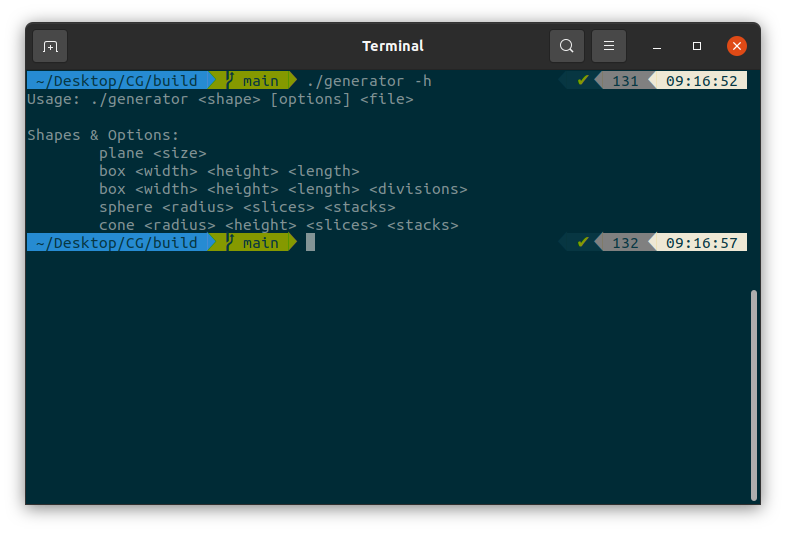
\includegraphics[width=.6\textwidth]{img/generator_h.png}
    \caption{Comando \textit{help} do \textit{generator}}
\end{figure}

\begin{figure}[H]
    \centering
    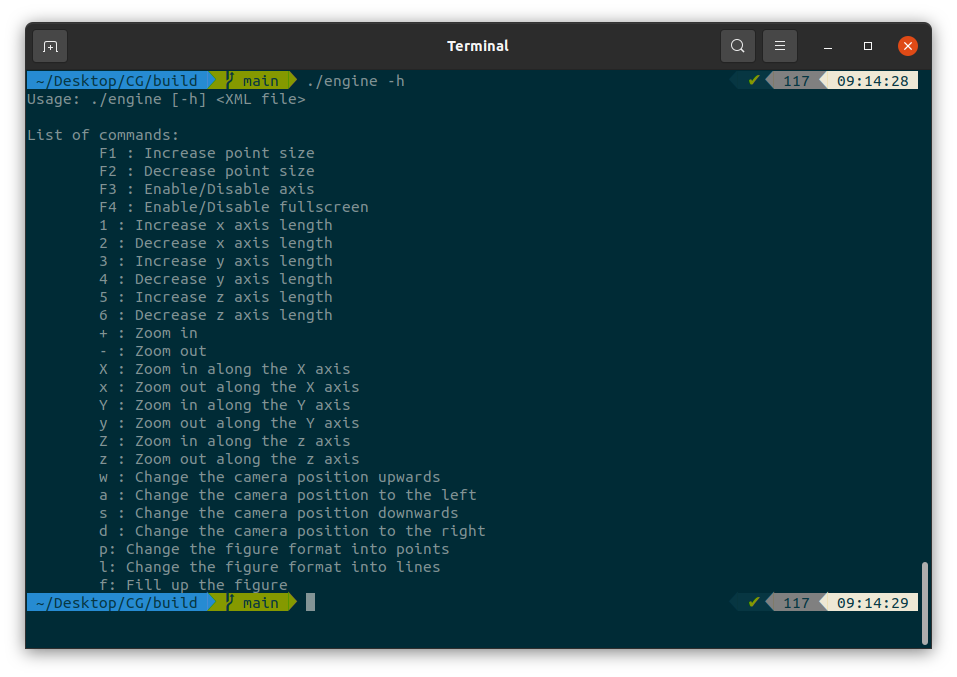
\includegraphics[width=.7\textwidth]{img/engine_h.png}
    \caption{Comando \textit{help} do \textit{engine}}
\end{figure}

\subsection{\textit{Generator}}

Tal como dito anteriormente, o \textit{generator} é responsável pelo cálculo das coordenadas dos 
pontos necessários para o desenho dos dos triângulos que compõem as diversas primitivas gráficas.

Neste módulo foram definidas 4 primitivas gráficas: plano, paralelepípedo, esfera e cone. Como 
tal, existiu a necessidade adotar algoritmos distintos em função da primitiva em questão, algoritmos
esses que serão discutidos a seguir.

O formato escolhido para representar cada um dos pontos gerados consiste de colocar um ponto por 
linha com as coordenadas $x$, $y$ e $z$, por esta ordem e separadas por um espaço. Assim, o conjunto
de pontos $(1, 0, 0)$, $(0, 1, 0)$ e $(0, 0, 1)$ seria representado como:

\begin{center}
\begin{tabular}{c}
\begin{lstlisting}
1 0 0
0 1 0
0 0 1
\end{lstlisting}
\end{tabular}
\end{center}

\subsection{\textit{Engine}}

O \textit{engine} é a aplicação responsável por receber o ficheiro de configuração de uma 
\textit{scene} em XML com todos os ficheiros que contém os modelos a ser carregados para serem
posteriomente gerados através do OpenGL. Cada ficheiro com modelos presentes no ficheiro de
configuração é analisado pelo programa para dele serem extraídos os vários pontos que
são depois adicionados a uma estrutura de dados adequada. 

Assim, é necessário percorrer todas as linhas destes ficheiros e guardar cada entrada como um 
ponto $(x, y, z)$ no espaço 3D.  Para isso, foi criada uma classe \texttt{Vertex} que representa
cada um destes pontos. Deste modo, cada entrada do ficheiro é instanciada como um objeto desta
classe, sendo esta posteriormente adicionada à lista de pontos a desenhar,
\texttt{std::vector<Vertex> vertices}.

Uma vez tendo os pontos necessários para o desenho dos triângulos que compõem diferentes 
primitivas, é, então, possível desenhar as figuras. Para tal, é necessário percorrer a estrutura
supracitada e desenhar cada um dos pontos invocando, para isso, funções do OpenGL.

De seguida, cada modelo é renderizado no ecrã, chamando a função \texttt{glVertex3f} para cada 
um dos seus pontos previamente carregados para memória e, por fim, inicia-se o \textit{main loop}
do GLUT. Desta forma, os modelos são carregados para memória apenas uma vez.

\begin{minted}{C++}
class Vertex {
        private:
        float _x, _y, _z;
        // (...)
};
\end{minted}

A título de exemplo, considerando os ficheiros \texttt{sphere.3d}, \texttt{coneup.3d} e 
\texttt{conedown.3d} gerados utilizando os comandos \texttt{./generator sphere 4 50 50}, 
\texttt{./generator cone 4 4 50 50}, e \texttt{./generator cone 4 -4 50 50},
respetivamente, e considerado o ficheiro XML \texttt{scene.xml} apresentado a seguir, o 
\textit{output} gerado pelo \textit{engine} é o seguinte:

\begin{minted}{XML}
<scene>
    <model file="sphere.3d" />
    <model file="coneup.3d" />
    <model file="conedown.3d" />
</scene>
\end{minted}

\begin{figure}[H]
    \centering
    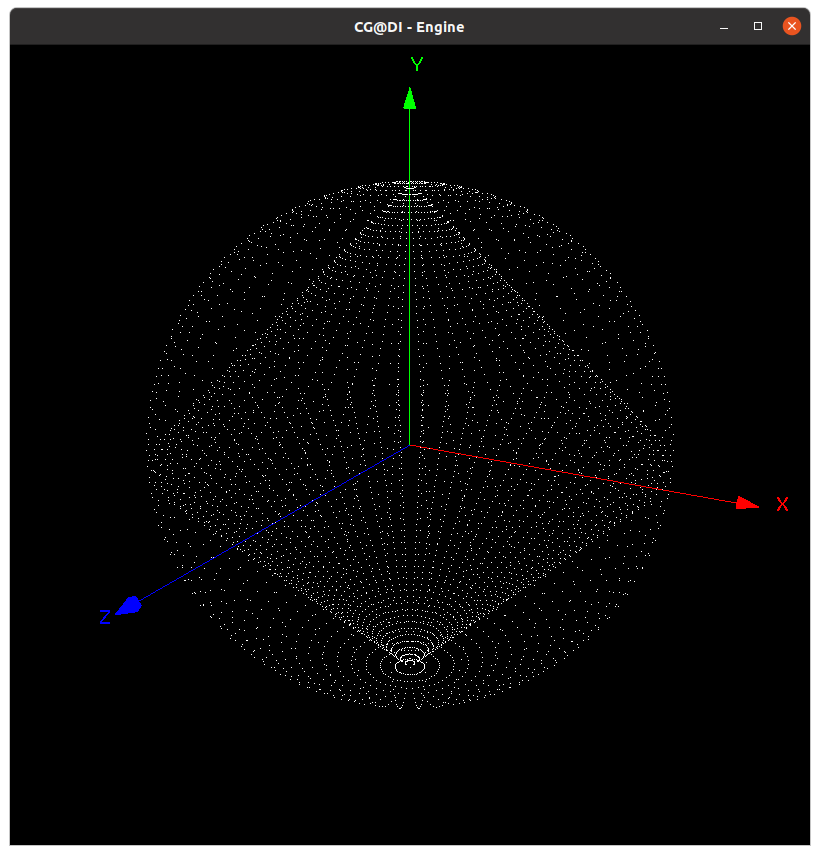
\includegraphics[width=.6\textwidth]{img/output_exemplo.png}
    \caption{\textit{Output} gerado pelo \textit{engine}}
\end{figure}


\pagebreak

\section{Primitivas Gráficas}

Para esta fase do trabalho prático foram desenhadas quatro primitivas gráficas, nomeadamente um 
plano, um cubo, uma esfera e um cone. Serão, em seguida, apresentados os algoritmos para o cálculo
dos vértices necessários para o desenho de cada uma destas primitivas.

\subsection{Plano}

Para a construção do plano, que pode ser interpretado como 2 triângulos, é necessário um 
argumento: a sua dimensão
(\texttt{size}).

Sabendo que um triângulo é definido por 3 vértices, verifica-se que 2 dos 4 vértices 
necessários à definição do um plano irão ser partilhados por ambos os triângulos. Sabendo também
que o plano está centrado na origem e como este é desenhado sobre o plano $XZ$, o valor de $y$ para
todos os pontos é constante e igual 0. Por fim, uma vez que se pretende que este
fique centrado na origem, é necessário dividir o comprimento passado como argumento 
(\texttt{size}) por dois de modo a obter as coordenadas em $X$ e $Z$ necessárias para formar
ambos os triângulos.

\begin{figure}[H]
    \centering
    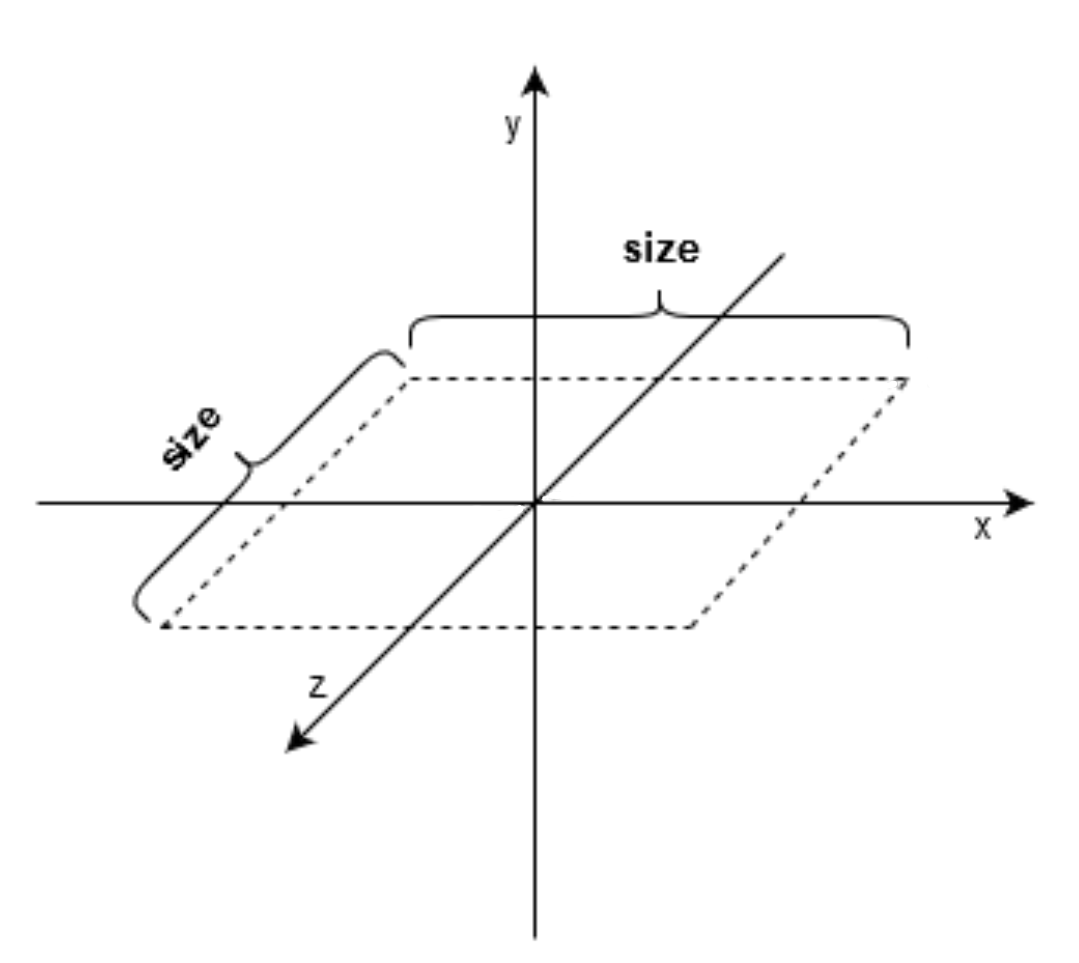
\includegraphics[width=.5\textwidth]{img/plane.png}
    \caption{Representação de um plano centrado na origem}
\end{figure}

Assim, tal como ilustrado na figura anterior, os vértices dos triângulos terão as seguintes
coordenadas:

$$\left(\frac{size}{2}, 0, \frac{size}{2}\right), \left(-\frac{size}{2}, 0, -\frac{size}{2}\right), 
\left(-\frac{size}{2}, 0, \frac{size}{2}\right)$$

\noindent e

$$\left(-\frac{size}{2}, 0, -\frac{size}{2}\right), \left(\frac{size}{2}, 0, \frac{size}{2}\right), 
\left(\frac{size}{2}, 0, -\frac{size}{2}\right)$$

\ \\

O resultado da renderização pode ser visto na figura seguinte:

\begin{figure}[H]
\centering
\begin{subfigure}{.5\textwidth}
    \centering
    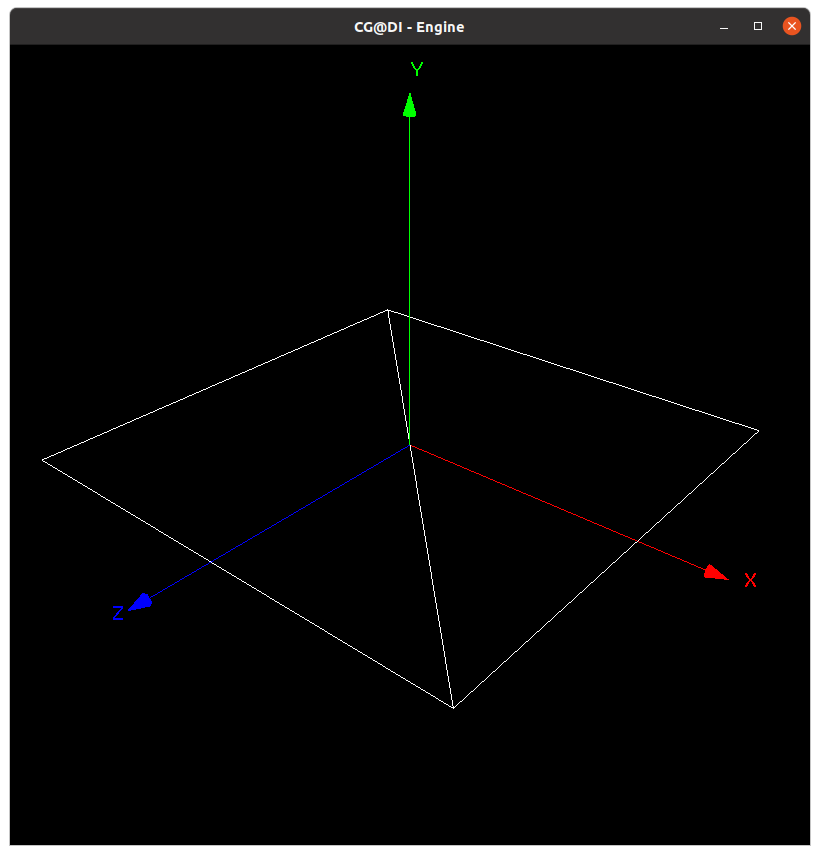
\includegraphics[width=\textwidth]{img/plano_linhas.png}
    \caption{Plano renderizado no modo \texttt{GL\_LINE}}
\end{subfigure}%
\begin{subfigure}{.5\textwidth}
    \centering
    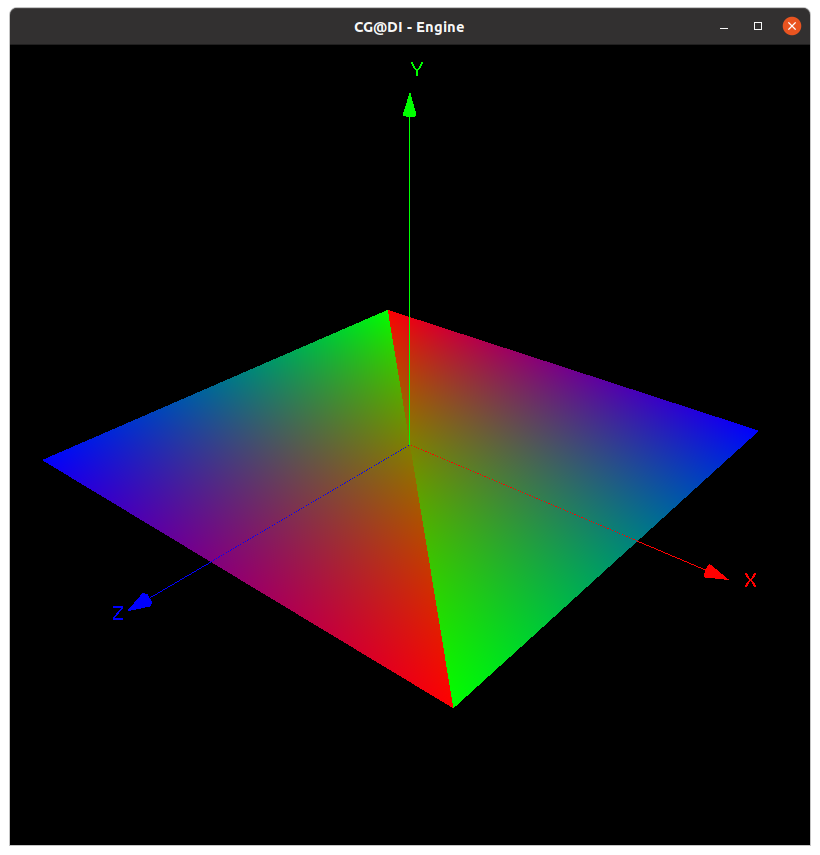
\includegraphics[width=\textwidth]{img/plano_preenchido.png}
    \caption{Plano renderizado no modo \texttt{GL\_FILL}}
\end{subfigure}
\caption{Plano com comprimento 8}
\end{figure}

\subsection{Paralelepípedo}

Um paralelepípedo é composto por 6 faces. Sendo assim, para a sua construção são necessários 
vários argumentos: o comprimento (\texttt{width}), a altura (\texttt{height}) e o comprimento
(\texttt{length}). Pode, opcionalmente, ser também passado como argumento o número de divisões em
cada face\footnote{Um paralelepípedo sem divisões nas faces pode ser visto como
um paralelepípedo com divisões tal que \texttt{divisions = 1}.} (\texttt{divisions}).

Tendo o paralelepípedo centrado na origem de forma a facilitar os cálculos, e sabendo que cada 
uma das faces é constituída por $divisions^2$ quadriláteros, e sendo cada um deles formado por dois
triângulos, é possível determinar o espaçamento entre cada um destes quadriláteros, espaçamento
esse que será utilizado para iterar sobre todo o sólido:

$$d_x = \frac{width}{divisions}$$
$$d_y = \frac{height}{divisions}$$
$$d_z = \frac{length}{divisions}$$

Desta forma, torna-se, então, possível calcular as coordenadas de todos os vértices necessários 
à construção do sólido. Tal como ilustrado na figura seguinte, e usando como exemplo um triângulo
da face frontal de um paralelepípedo, teríamos as seguintes coordenadas, onde $i$ e $j$ serão
variáveis que permitem iterar ao longo das faces:

\textbf{Vértice A:} $$\left(d_x\times i - \frac{width}{2}, d_y \times j - \frac{height}{2}, 
\frac{length}{2} \right)$$

\textbf{Vértice P:} $$\left(d_x\times i - \frac{width}{2} + d_x, d_y \times j - \frac{height}{2}, 
\frac{length}{2} \right)$$

\textbf{Vértice R:} $$\left(d_x\times i - \frac{width}{2}, d_y \times j - \frac{height}{2} + d_y, 
\frac{length}{2} \right)$$

\begin{figure}[H]
    \centering
    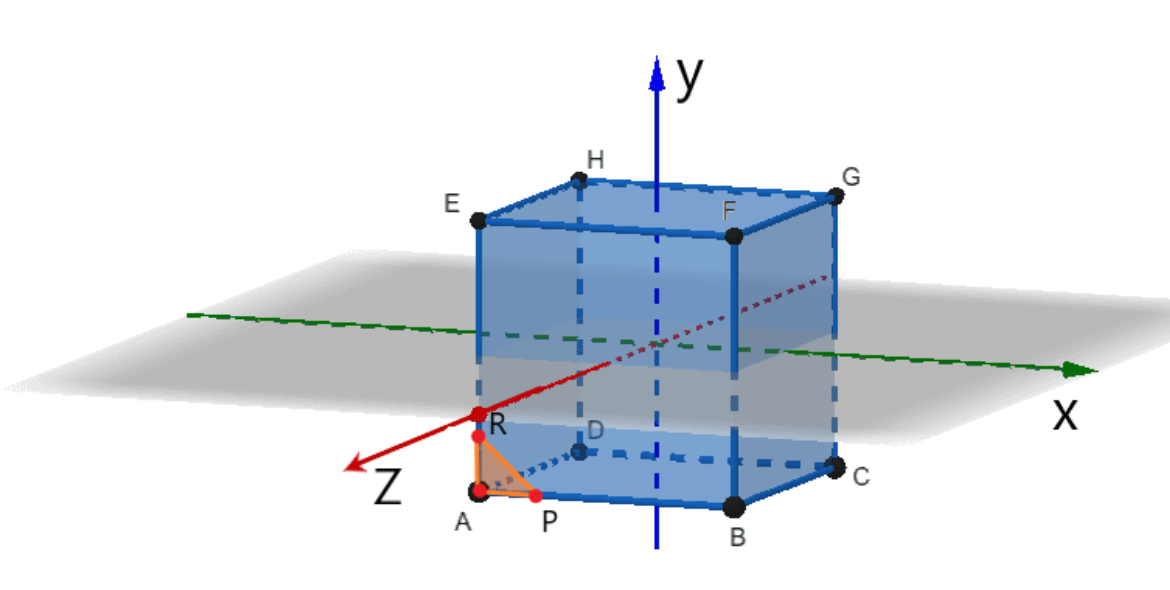
\includegraphics[width=.6\textwidth]{img/paralelepipedo.png}
    \caption{Representação de um paralelepípedo centrado na origem}
\end{figure}

O resultado da renderização pode ser visto na figura seguinte:

\begin{figure}[H]
\centering
\begin{subfigure}{.5\textwidth}
    \centering
    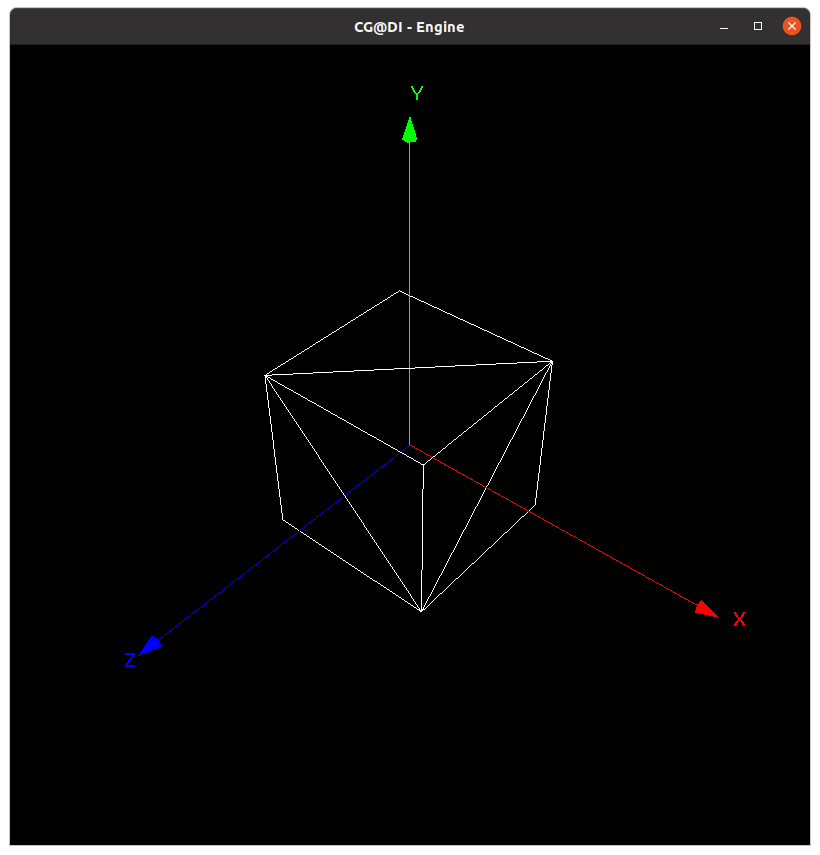
\includegraphics[width=\textwidth]{img/box_linhas.png}
    \caption{Paralelepípedo sem divisões renderizado \\no modo \texttt{GL\_LINE}}
\end{subfigure}%
\begin{subfigure}{.5\textwidth}
    \centering
    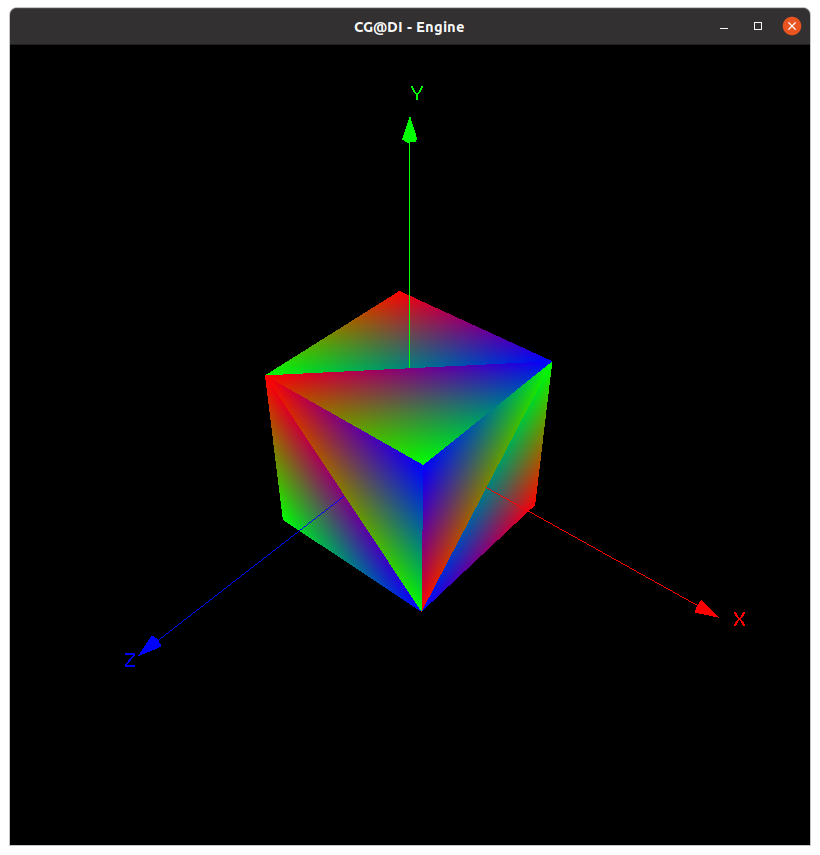
\includegraphics[width=\textwidth]{img/box_preenchida.png}
    \caption{Paralelepípedo sem divisões renderizado no modo \texttt{GL\_FILL}}
\end{subfigure}
\caption{Paralelepípedo sem divisões, com dimensões $3\times3\times3$}
\end{figure}

\begin{figure}[H]
\centering
\begin{subfigure}{.5\textwidth}
    \centering
    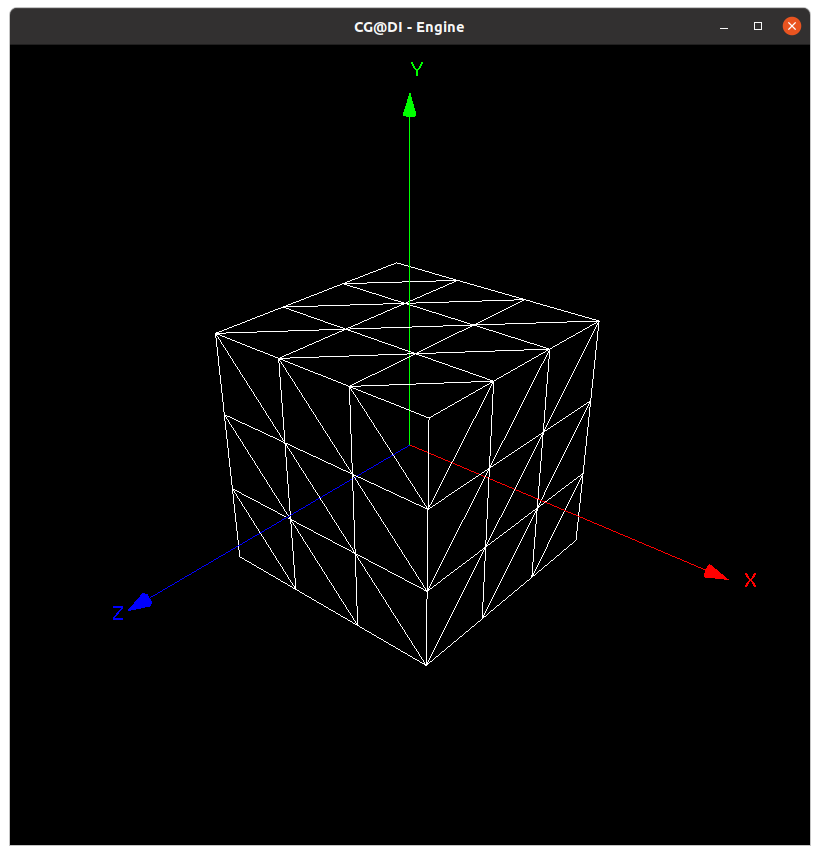
\includegraphics[width=\textwidth]{img/box_div_linhas.png}
    \caption{Paralelepípedo com divisões nas faces \\renderizado no modo \texttt{GL\_LINE}}
\end{subfigure}%
\begin{subfigure}{.5\textwidth}
    \centering
    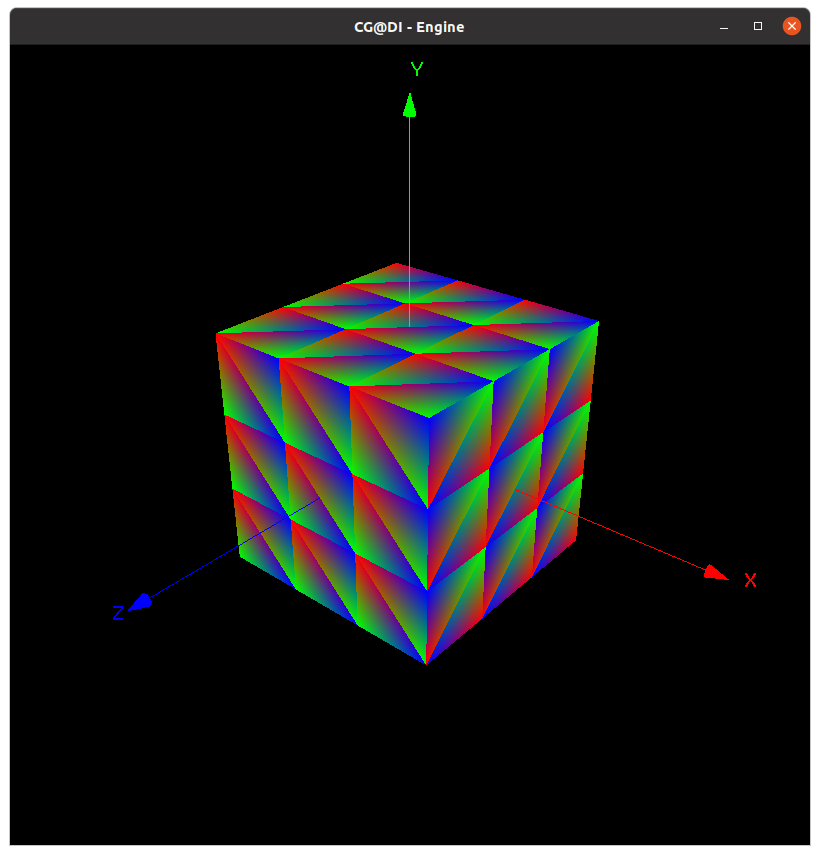
\includegraphics[width=\textwidth]{img/box_div_preenchida.png}
    \caption{Paralelepípedo com divisões nas faces \\renderizado no modo \texttt{GL\_FILL}}
\end{subfigure}
\caption{Paralelepípedo de dimensões $4\times4\times4$, e 3 divisões por face}
\end{figure}

\subsection{Esfera}

Para a criação da esfera são utilizadas coordenadas esféricas de modo a facilitar o cálculo 
das coordenadas de cada um dos pontos. Deste modo, são necessárias duas variáveis para representar
os dois ângulos $\alpha$ e $\beta$, representados na figura que se segue, em função dos quais serão
expressas as coordenadas de cada ponto, e que serão atualizadas em cada iteração.

Uma esfera pode ser dividida em \textit{stacks} e \textit{slices}, que serão usadas para iterar à 
volta da mesma. A interseção entre uma \textit{slice} e uma \textit{stack} forma um retângulo,
composto por dois triângulos.

\begin{figure}[H]
\centering
\begin{subfigure}{.5\textwidth}
    \centering
    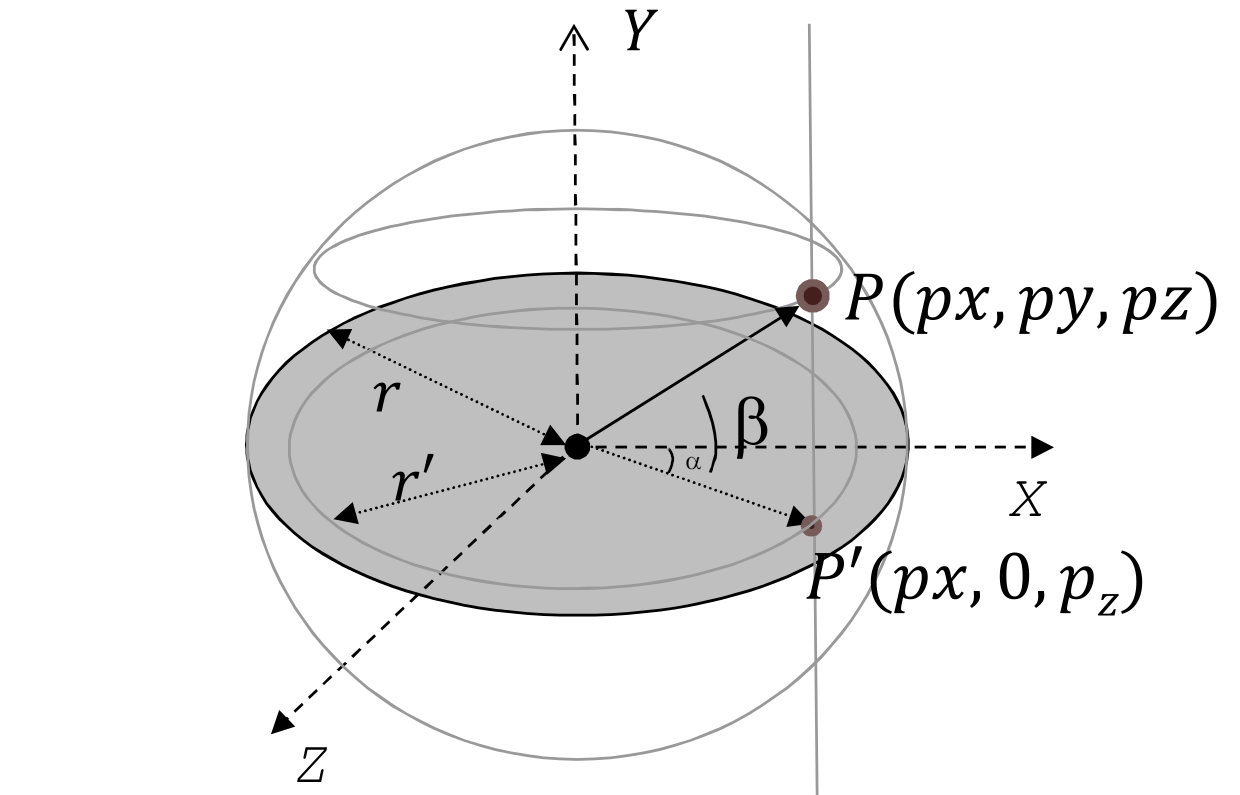
\includegraphics[width=\textwidth]{img/spherical.png}
    \caption{Sistema de coordenadas esféricas}
    \label{fig:coords}
\end{subfigure}%
\begin{subfigure}{.5\textwidth}
    \centering
    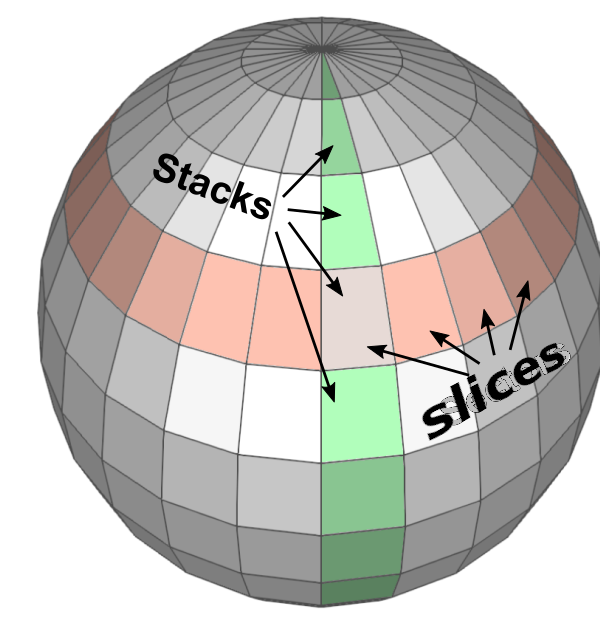
\includegraphics[width=.6\textwidth]{img/gl_sphere02.png}
    \caption{\textit{Stacks} e \textit{Slices}}
\end{subfigure}
\caption{Geometria de uma esfera}
\end{figure}

\pagebreak

Usando coordenadas esféricas, podemos facilmente obter as coordenadas cartesianas para guardar 
posteriormente nas respetivas estruturas de dados. Analisado a figura \ref{fig:coords}, e
considerando os ângulos $\alpha$ e  $\beta$, podemos obter as coordenadas de qualquer ponto sobre
a esfera, sendo que para determinar as coordenadas do ponto $P$ para o eixo dos $X$
basta fazer o produto do cosseno do ângulo $\alpha$ com o cosseno do ângulo $\beta$ e multiplicar 
estes dois fatores pelo raio da esfera. Para o eixo dos $Z$ o raciocínio é semelhante, 
sendo que agora basta fazer o produto do seno do ângulo $\alpha$ com o cosseno do ângulo 
$\beta$ e novamente multiplicando pelo o raio da esfera. Por fim, para obter o eixo dos $Y$, basta 
multiplicar o seno do ângulo $\beta$ com o raio da esfera e obtemos diretamente a coordenada $Y$.

Como forma de exemplo podemos observar que para calcular o ponto $P'$ bastava usar o cosseno de 
$\alpha$ para a coordenada em $X$, o seno de $\beta$ para a coordenada em $Z$ e simplesmente
igualar a coordenada em $Y$ a zero visto que estamos no plano $XZ$, no qual a coordenada $y$
toma sempre o valor zero. Usando agora o primeiro cálculo para calcular este ponto $P'$:

\begin{equation*}
\begin{cases}
x = \cos\alpha \times \cos\beta \times r \\
y = \sin\beta \times r \\
z = \sin\alpha \times \cos\beta \times r
\end{cases}
\end{equation*}

Como o ângulo $\beta$ é igual a 0, anulando os senos e cossenos da fórmula, temos como resultado 
a previsão inicial:

\begin{equation*}
\begin{cases}
x = \cos\alpha \times 1 \times r = \cos\alpha \times r\\
y = 0 \times r = 0 \\
z = \sin\alpha \times 1 \times r = \sin\alpha \times r
\end{cases}
\end{equation*}

Atendendo ao número de \textit{stacks} e \textit{slices}, é possível calcular dois 
deslocamentos: o deslocamento horizontal,
$d_\alpha$, entre \SI{0}{\radian} e \SI{2\pi}{\radian}, e o deslocamento vertical, $d_\beta$, entre 
\SI{0}{\radian} e
\SI{\pi}{\radian}.

$$d_\alpha = \frac{2\pi}{slices}$$
$$d_\beta = \frac{\pi}{stacks}$$

\

Assim, e com estes deslocamentos, podemos proceder ao cálculo dos vertices, tendo em 
consideração que o ângulo $\alpha$ é incrementado a cada iteração no valor de $d_{\alpha}$ e, 
quando este atingir o valor de \SI{2\pi}{\radian} (\textit{i.e.} quando der uma volta completa
em torno da esfera), é, então, incrementado o angulo $\beta$, recorrendo ao valor $d_{\beta}$,
e $\alpha$ é inicializado a partir do 0, novamente, e é mais uma vez percorrida a esfera 
horizontalmente, até que ângulo $\beta$ atinja o valor de \SI{\pi}{\radian}.

\pagebreak
O resultado da renderização pode ser visto na figura seguinte:

\begin{figure}[H]
\centering
\begin{subfigure}{.5\textwidth}
    \centering
    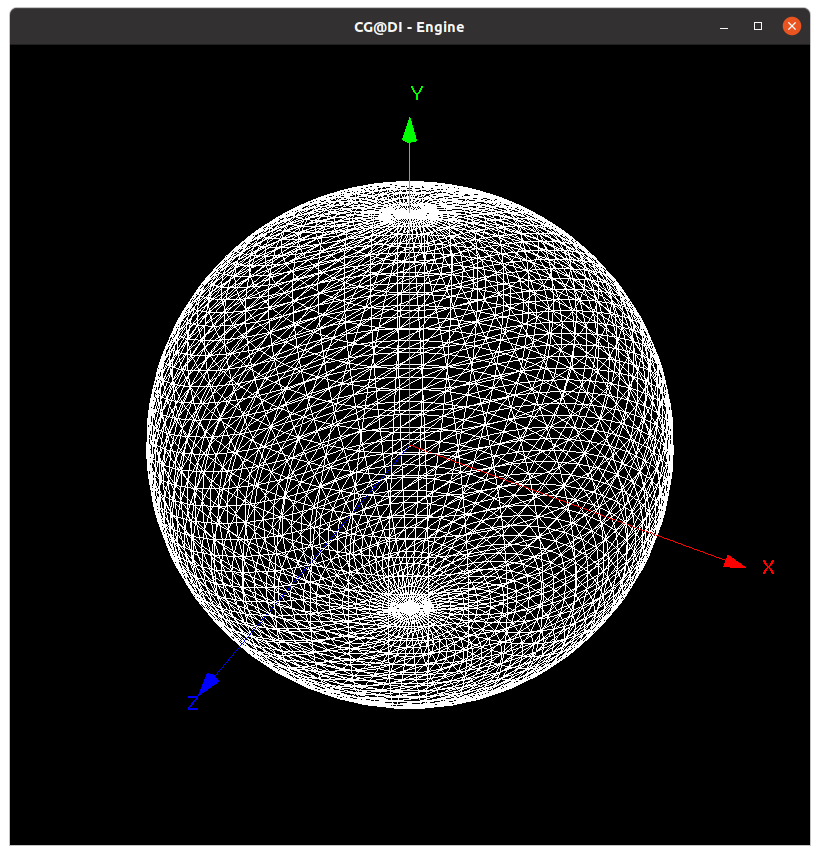
\includegraphics[width=\textwidth]{img/esfera_linhas.png}
    \caption{Esfera renderizada no modo \texttt{GL\_LINE}}
\end{subfigure}%
\begin{subfigure}{.5\textwidth}
    \centering
    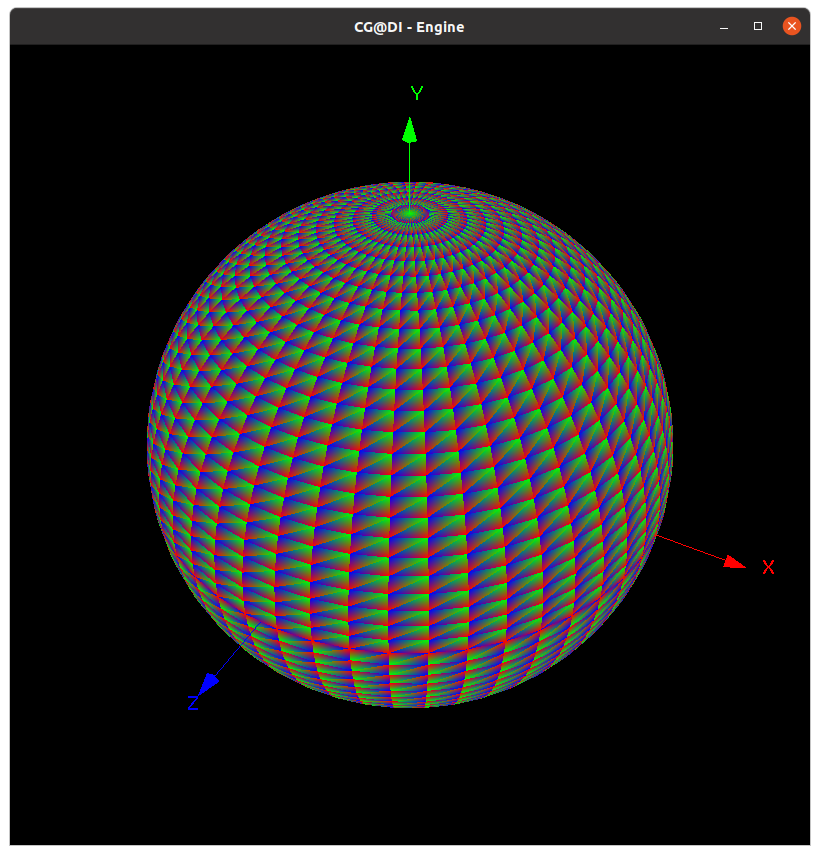
\includegraphics[width=\textwidth]{img/esfera_preenchida.png}
    \caption{Esfera renderizada no modo \texttt{GL\_FILL}}
\end{subfigure}
\caption{Esfera de raio 8, construída com 50 \textit{slices} e 50 \textit{stacks}}
\end{figure}

\subsection{Cone}

Para desenhar um cone é necessário saber o seu raio (\texttt{radius}), a sua
altura (\texttt{height}), o número de \textit{slices} (\texttt{slices}) e o número de 
\textit{stacks} (\texttt{stacks}).

O algoritmo para o desenho de um cone introduz cálculos trigonométricos para o cálculo das 
coordenadas dos vértices, em função dos mesmos ângulos $\alpha$ e $\beta$ referidos anteriormente. 
A diferença do cone para a esfera reside no facto de o ângulo $\alpha$ estar continuamente a
decrescer à medida que percorremos o eixo $Y$, isto sabendo que o vetor da origem $O$ ao vértice
do cone está paralelo e com o mesmo sentido do eixo positivo $Y$. Dividindo então este ângulo
inicial $\alpha$ pelo número de \textit{slices}, obtemos o deslocamento radial $\Delta\alpha$ que 
permitirá decrementar o ângulo $\alpha$ a cada camada do cone. Ao decrementar este ângulo, podemos
facilmente obter as coordenadas dos pontos utilizando um raciocínio análogo ao da construção
da esfera. 

\pagebreak 
O resultado da renderização pode ser visto na figura seguinte:

\begin{figure}[H]
\centering
\begin{subfigure}{.5\textwidth}
    \centering
    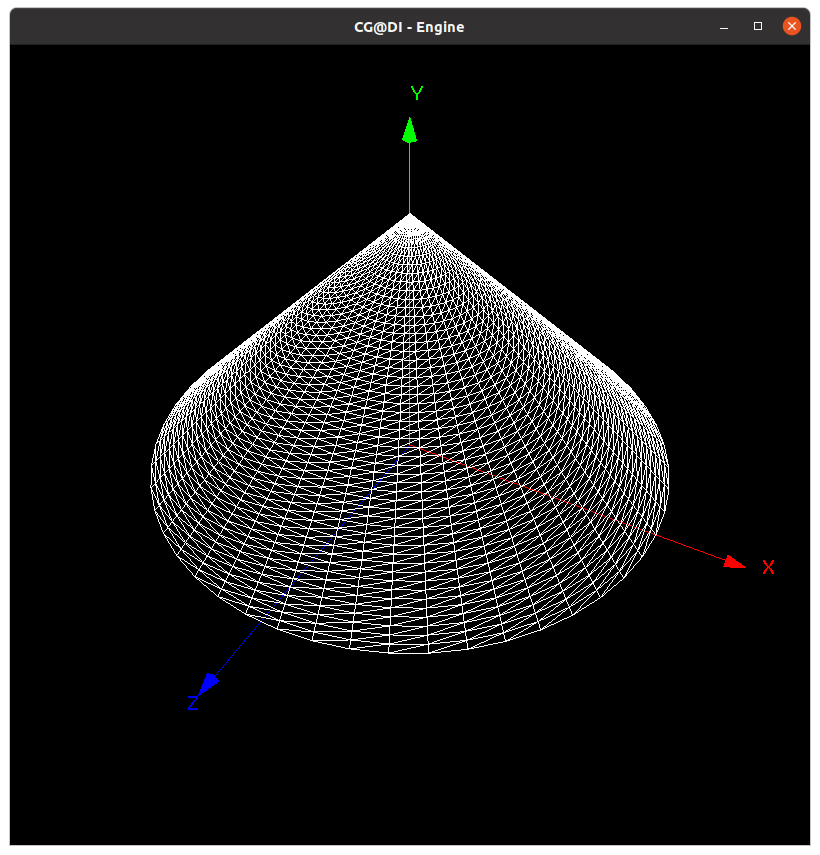
\includegraphics[width=\textwidth]{img/cone_linhas.png}
    \caption{Cone sem divisões renderizado no \\modo \texttt{GL\_LINE}}
\end{subfigure}%
\begin{subfigure}{.5\textwidth}
    \centering
    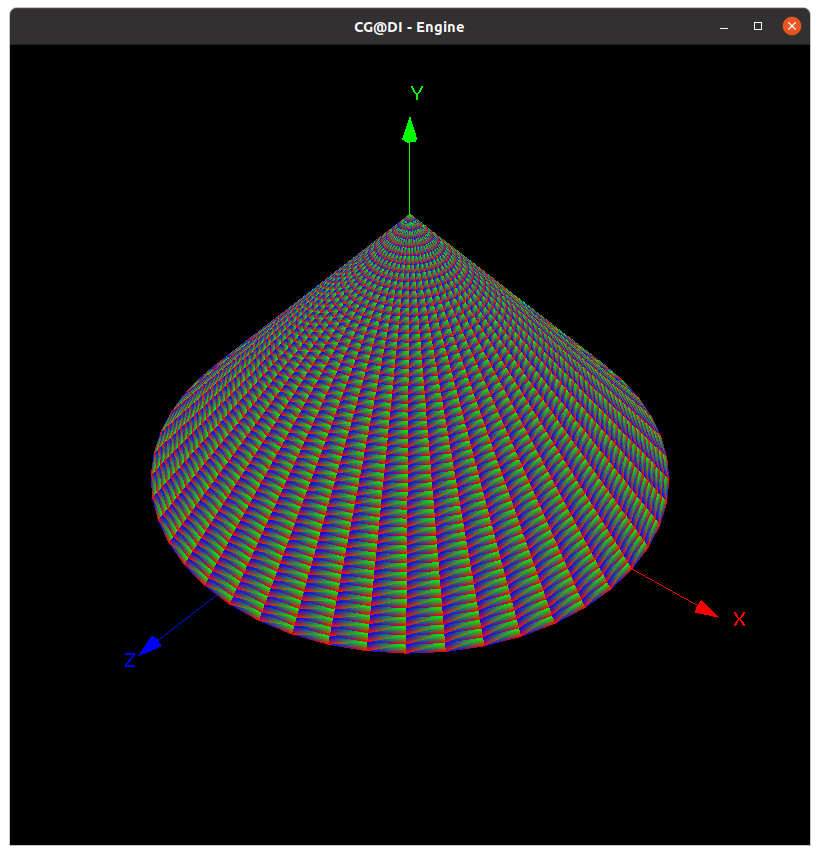
\includegraphics[width=\textwidth]{img/cone_preenchido.png}
    \caption{Paralelepípedo sem divisões renderizado no modo \texttt{GL\_FILL}}
\end{subfigure}
\caption{Cone de raio 4 e altura 4, construído com 50 \textit{slices} e 50 \textit{stacks}}
\end{figure}

\section{Conclusão}

A elaboração desta primeira fase do trabalho prático permitiu a consolidação de conhecimentos 
relativos ao OpenGL e GLUT e, ao mesmo tempo, a linguagem de programação de C++, e até mesmo 
relembrar certos aspetos no âmbito da geometria.

Fazendo uma análise geral ao trabalho desenvolvido ao longo desta primeira fase, conclui-se que 
foram cumpridos todos os objetivos que foram propostos.

Como trabalho futuro gostaríamos de implementar outras primitivas no \textit{generator}, como por
exemplo  o \textit{torus}, assim como a implementação de uma câmara
\textit{FPS -- First-Person Shooter} no \textit{engine}.

\end{document}
